\chapter{Introduction}

\noindent{}\rOne{Changes from the first review are red.}

\noindent{}\rTwo{Changes from the second review are blue.}

\noindent{}\rThree{Changes from the third review are ForestGreen.}

% https://www.scribbr.com/dissertation/introduction-structure/

% Your topic, in context: what does your reader need to know to understand your thesis dissertation?
% Your focus and scope: what specific aspect of the topic will you address?
% The relevance of your research: how does your work fit into existing studies on your topic?
% Your questions and objectives: what does your research aim to find out, and how?
% An overview of your structure: what does each section contribute to the overall aim?

\noindent{}Every image we see creates a unique signature in our brain. But how accurately can we decode and reconstruct what someone has seen, purely from their brain activity? Recent insights in brain decoding research using functional magnetic resonance imaging (fMRI) allow us to translate complex neural patterns into visual images\cite{shenDeepImageReconstruction2019,scottiMindEye2SharedSubjectModels2024,ozcelikNaturalSceneReconstruction2023}. \rTwo{Yet, a major problem in this field is that oftentimes images that are out of distribution (OOD) from the training data can only be poorly reconstructed\cite{kamitaniDecodingVisualSubjective2005,shirakawaSpuriousReconstructionBrain2024}. In this thesis, the question should be answered, if the issue of OOD generalisation can be better understood and the reconstruction of these samples can be improved.} \rTwo{The overarching goal of the research on image reconstruction from brain activity} is to find a way to reconstruct all possible images from brain activity, including those that were not shown to a subject during data acquisition. Shirakawa et al.~\cite{shirakawaSpuriousReconstructionBrain2024} found that supposed recent successes in image reconstruction~\cite{ozcelikNaturalSceneReconstruction2023,scottiMindEye2SharedSubjectModels2024} are likely only a consequence of overlapping concepts in the training and test data, and not a sign of generalisation. Furthermore, they argue that high diversity in the training data may help to get closer to true generalisation in image reconstruction. Yet, a major problem in this field is the amount of data that can be collected from each participant: in order to train brain activity decoder algorithms for image reconstruction, multiple hours of recording are needed~\cite{horikawaGenericDecodingSeen2017,gifford7TFMRIDataset2025,hebartTHINGSdataMultimodalCollection2023}, costing both lots of time and money. 

Therefore, in this paper, the influence of the diversity of training images on the quality of image reconstruction from brain activity is investigated in three different experiments \rTwo{that require no additional data to be recorded}. The experimental data was previously collected in other studies and follows the study design of Horikawa et al.~\cite{horikawaGenericDecodingSeen2017}. The first experiment attempts to create subsets from the training data that are maximised according to their diversity and should therefore perform better than randomly selected data. In the second experiment, alternative captions (short descriptions of the training images) are generated that focus on different aspects of the images and are used in the training for image reconstruction. In the third experiment, the training images are enriched with semantic information about the depicted objects using perturbations, so that they either contain more or less semantic information.

This thesis is divided into four parts. This introduction is followed by an explanation of the background necessary to have an understanding of the work, including the development of algorithms for reconstructing images from brain activity and the influence of diversity in the training of machine learning algorithms. The second part contains a description of the methodology used for all the experiments in this thesis as well as a validation of the reconstruction algorithms used without further modifications. The following main part of the thesis describes the three experiments. Each section on an experiment itself follows a similar structure to the whole thesis: the theoretical background of the experiment is described, the methodology is explained, the results are listed and critically discussed. The experimental section is followed by a discussion of the results in the broader context of the influence of data diversity on image reconstruction in general. Finally, implications for future research are given.


\section{Background}

\subsection{Brain decoding and image reconstruction}

It has long been known that the visual system contains neurons that respond to various stimuli, such as object orientation, movement or color~\cite{grill-spectorHUMANVISUALCORTEX2004}. Functional magnetic resonance imaging (fMRI) has enabled noninvasive examination of these neural regions in greater detail. The visual cortex follows two main principles: hierarchical processing and functional specialization. Hierarchical processing indicates that increasingly complex features are encoded progressively from primary visual area V1 up to area V4. Functional specialization refers to parallel hierarchical pathways, commonly known as the `where' and `what' pathways, which process spatial information and object identification, respectively~\cite{grill-spectorHUMANVISUALCORTEX2004,ungerleiderWhatWhereHuman1994}. Specific regions within the cortex have been identified to respond preferentially to different stimulus types; for instance, the fusiform face area (FFA) is specialized for faces~\cite{kanwisherFusiformFaceArea1997}, whereas the parahippocampal place area (PPA) predominantly responds to scenes rather than individual objects or faces~\cite{epsteinCorticalRepresentationLocal1998}. Further, cortical regions responding specifically to shape features have also been described~\cite{kourtziCorticalRegionsInvolved2000}. Many studies focus on broad cortical modules (e.g. V1), but detailed insights into stimuli (e.g.\ the region within v1 that codes for horizontal edges) require finer resolution. In order get a more granular view on brain regions, the voxels that the fmri measures can be analysed. Although the voxel size is still not granular enough to find single neurons that code for example for a specific orientation of stimuli, the `average' activation of the neurons within a voxel might lean towards a specific orientation of a seen stimulus~\cite{kamitaniDecodingVisualSubjective2005} and thus the voxels can contain this very granular information in an indirect way. When investigating brain regions, one can differentiate between encoding and decoding models. Encoding models try to predict brain activity depending on a given stimulus, decoding does the exact opposite: depending on measured brain activity, characteristics of a stimulus are supposed to be predicted~\cite{naselarisEncodingDecodingFMRI2011}. For reconstructing visual stimuli from measured brain activity, decoding models are essential. Decoding models typically employ linear classifiers due to their effectiveness in cases where the amount of data is limited. Although neural interactions within the brain may be nonlinear, revealing these interdependencies through more complex models requires extensive datasets, which is usually not feasible in fMRI experiments (both due to the high recording effort and the granularity of the recorded data). Early influential decoding work by Kamitani and Tong~\cite{kamitaniDecodingVisualSubjective2005} demonstrated that the orientation of edges (from eight possible orientations) could be predicted from fMRI activity from the activity early visual areas (V1 and V2). 
Despite orientation columns in the visual areas likely being smaller than individual voxels, ensemble decoding methods successfully extracted meaningful orientation information, that enabled the prediction of the orientation of seen stimuli. Advancing further, Miyawaki et al.~\cite{miyawakiVisualImageReconstruction2008} introduced a method for image reconstruction, successfully predicting visual patterns composed of 10$\times$10 pixel patches (resulting in $2^{100}$ possible states). They trained multiple local translators with slightly different features (for example single pixels or $2\time1$ pixel rectangles) that were then used together in an ensemble approach to reconstruct the shown stimuli. Like previous studies, Miyawaki et al.~ predominantly relied on low-level visual information from V1 and V2, as higher-level areas (V3 and V4) had minimal influence on the reconstruction. 
A limitation arising from this body of work is the predominant use of low-level visual information from early cortical regions, thus restricting reconstructions primarily to low-level features (like contours and textures) without capturing much of the semantic meaning. Addressing this limitation, Horikawa et al.~\cite{horikawaGenericDecodingSeen2017} developed an approach that was able to incorporate the influence of higher cortical regions into the translator. They were able to create a generic object translator, which enabled the prediction of diverse object categories from brain activity without relying on having a definite set of objects that was learned in the training data. Using sparse linear regression, they predicted feature vectors from different layers of convolutional neural networks (CNNs). This approach demonstrated a correspondence between the hierarchical processing within the human brain and CNN hierarchies: low-level CNN features were predicted from early visual regions (V1, V2), whereas high-level CNN features correlated with activity in higher visual regions (V4, LOC, PPA, FFA).

Now that features of deep learning models, it is possible to integrate higher brain structures into the decoding process. In this way, a general reconstruction of visual stimuli can be pursued, which is not only based on low-level image features, but also, for example, on semantically semantic categories (e.g.\ in~\cite{shenDeepImageReconstruction2019,ozcelikNaturalSceneReconstruction2023}). Shirakawa et al.~\cite{shirakawaSpuriousReconstructionBrain2024} describe the general workflow used by modern reconstruction algorithms. This pipeline is illustrated in Figure~\ref{fig:recon_pipeline}. Image Reconstruction essentially consists of two steps: first, a decoder is used to map the brain data onto latent features. \rOne{The word `decoder' is however used for many different concepts. Thus in this work, the model that translates the brain activity to some latent space will be called translator instead}. These latent features may, as in Horikawa et al.~\cite{horikawaGenericDecodingSeen2017}, contain aggregated information about the low-level and high-level visual information. Typically, a linear model is used for the translator, which can learn to predict the features robustly and with little data from brain activity. The latent features are then converted into an image in a second step using a generator module, which can use different techniques such as diffusion models~\cite{xuVersatileDiffusionText2024,ozcelikNaturalSceneReconstruction2023} or generative adversarial networks (GANs). These generative models are usually too complex to be trained with the small amount of recorded brain activity. Therefore, pre-trained models are used here to generate images from the previously predicted latent features.

\begin{figure}[ht]
    \centering
    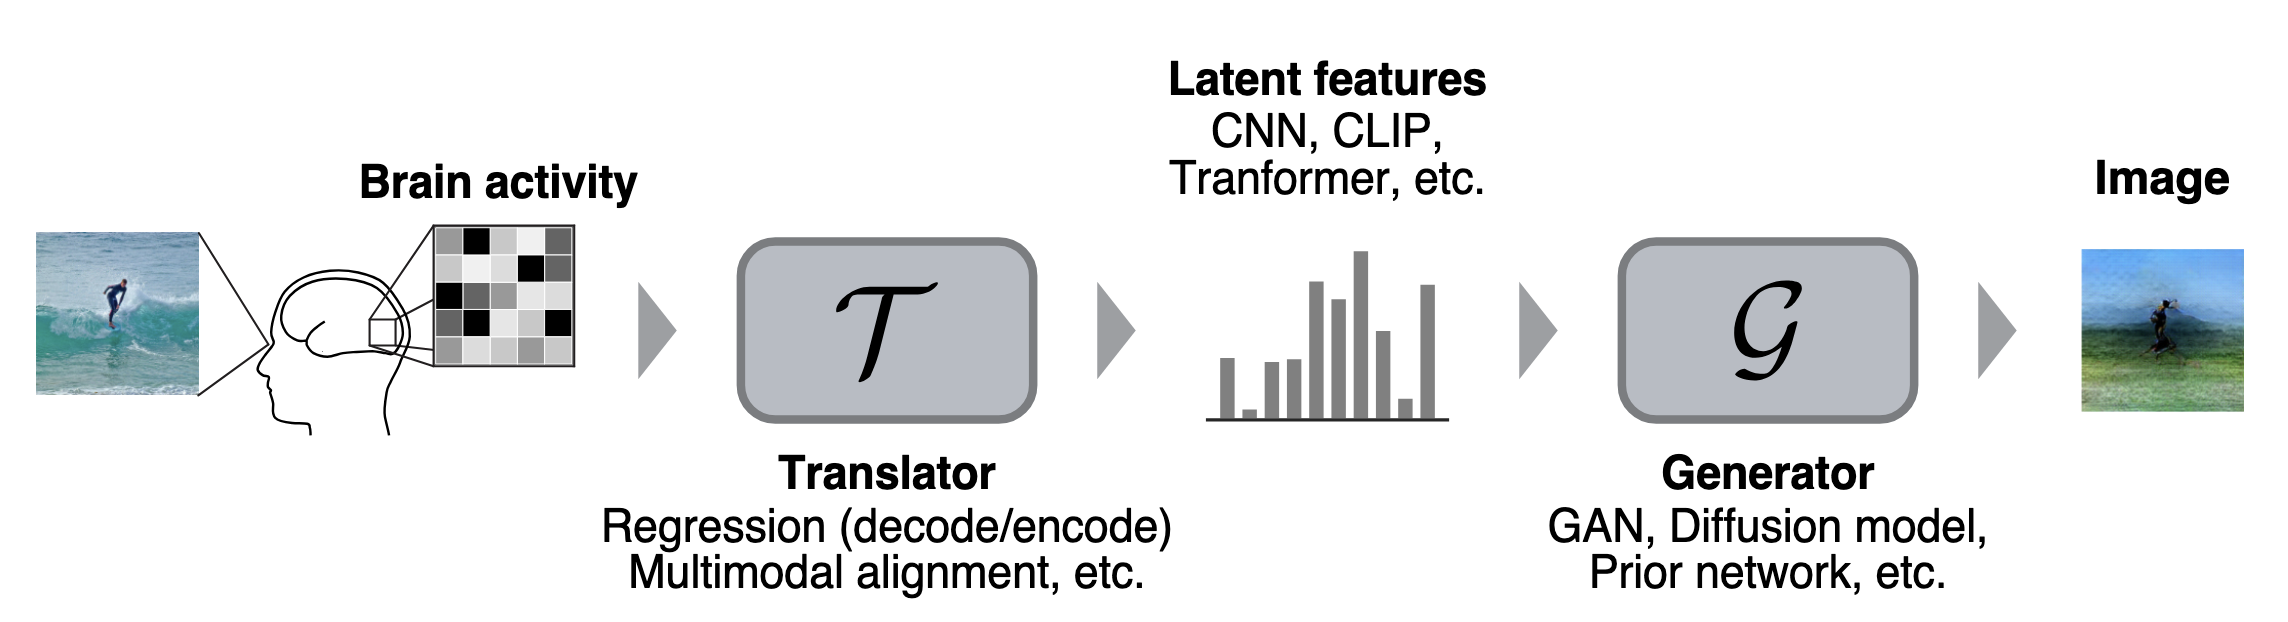
\includegraphics[width=0.8\textwidth]{plots/01_background_shirakawa_recon_pipeline.png}
    \caption[General Reconstruction Pipeline]{Visualization of the general Reconstruction Pipeline taken from Shirakawa et al.~\cite{shirakawaSpuriousReconstructionBrain2024}}\label{fig:recon_pipeline}
\end{figure}

One algorithm using this approach is the iterative Convolutional Network algorithm (iCNN), first described by Shen et al.~\cite{shenDeepImageReconstruction2019}. They adopted the method introduced by Horikawa et al.~\cite{horikawaGenericDecodingSeen2017} to predict hierarchical features of a deep neural network based on brain activity and subsequently used these features to reconstruct images that the participants have seen. Specifically, Shen et al.\ used a VGG-19 network that was pre-trained on ImageNet, to obtain features from the training images. Then a sparse linear regression was trained to predict these features from the brain activity. Then, for two different test datasets, the trained \rOne{translator} predicted the test features from the brain activity. Backpropagation is used to adjust the pixels in multiple steps to minimise the loss between the predicted features and the features, that the pixels produce in the vgg-19 network. In addition, an optional deep generator network was introduced to act as an image prior to improve the naturalness of the reconstructed images. Using this approach, Shen et al.\ successfully reconstructed both natural and artificially generated test images, effectively exploiting information from higher cortical structures. The iCNN has been used successfully to study the influence of attention on ambiguous stimuli. Horikawa et al.~\cite{horikawaAttentionModulatesNeural2022} showed two superimposed images in an experiment. Subjects were asked to focus on one of the images, and the image on which attention was focused could be successfully reconstructed. This shows that the iCNN can also be used to map attention-modulated top-down processes and does not only depend on the actual visual properties of an image. Cheng et al.~\cite{chengReconstructingVisualIllusory2023} used images that created optical illusions so that people perceived lines that were not actually present. These perceived (non-existent) features of the images could also be successfully reconstructed using the algorithm.

In addition to the iCNN, which reconstructs images through iterative pixel-space adaptation, a second class of algorithms relies on diffusion-based image generation~\cite{takagiHighResolutionImageReconstruction,ozcelikNaturalSceneReconstruction2023,scottiMindEye2SharedSubjectModels2024}. Typically, these methods also first map brain activity into a latent feature space using translation models like linear regression. Subsequently, a pre-trained diffusion model generates the images from these latent features. The Brain-Diffuser algorithm by Ozcelik et al.~\cite{ozcelikNaturalSceneReconstruction2023} uses three linear ridge regression-based~\cite{hoerlRidgeRegressionBiased1970} translators, each converting brain activity into distinct feature spaces: latent features from a Very Deep Variational Autoencoder (VDVAE)\cite{childVeryDeepVAEs2020},  CLIP Vision features and CLIP Text features~\cite{radfordLearningTransferableVisual2021}. Initially, the VDVAE is used to reconstruct the basic image structure with limited detail. Subsequently, the CLIP Text and CLIP Vision features enhance the image by adding semantic and visual details. These three types of features are used to guide the versatile diffusion algorithm~\cite{xuVersatileDiffusionText2024}, which first uses the initially reconstructed VDVAE image as a baseline and conditions it in an image-to-image diffusion process using the CLIP Vision and CLIP Text features. Using the Natural Scenes Dataset (NSD)~\cite{allenMassive7TFMRI2022}, Ozcelik et al.\ demonstrated that their multi-stage algorithm Brain-Diffuser effectively reconstructs both low-level attributes (e.g., shape and color) using the VDVAE and high-level semantic content from brain activity using the CLIP Features, successfully reconstructing the original images shown to test subjects.

\subsection{Data diversity}


Shirakawa et al.~\cite{shirakawaSpuriousReconstructionBrain2024} have further investigated the current image reconstruction methods and in particular diffusion-based approaches. It turned out that the good performance of the reconstruction was largely due to the fact that there is a high semantic overlap between the training and test data in the NSD dataset. In a critical review, they found that valid images could sometimes be reconstructed even with randomised brain activity. By clustering the training and test data in the CLIP space, they showed that only a relatively small number of clusters could be found in the training data (e.g. aeroplanes or dogs), and that these clusters overlapped considerably between training and test data. In a theoretical simulation-based analysis, they showed that the models (e.g.\ linear regression) used to translate brain activity tend to map all test data onto the subspace defined by the training data (and this fact could be even more true for nonlinear models). In the example of image reconstruction, this would mean that arbitrary brain activity would always be mapped to the subspace of the training data (i.e.\ images that are similar to those that are similar to the training data). The authors call this phenomenon output dimension collapse. Output dimension collapse explains why even random brain activity may produce valid reconstructions, and why out-of-distribution generalisation (e.g. reconstruction of concepts not present in the training data) can only work to a limited extent with the limited diversity of the training data. Due to the  output dimension collapse, the regression degenerates into a kind of classification of the concepts present in the training data set. In a further study with simulated data, the authors investigate under which circumstances true out-of-distribution generalisation becomes possible. They found that it is sufficient if there are enough clusters in the training data to span the entire output space (i.e.\ a linear increase in training data with respect to the number of output dimensions), so that it is not absolutely necessary to densely fill the entire output space with training data (i.e.\ an exponential increase in training data with respect to the number of output dimensions). These findings highlight the importance of diversity in training data when attempting to reconstruct arbitrary visual stimuli from brain activity.

At the same time, it is difficult to define which clusters in the training data are necessary to cover the entire image space (i.e.\ all images that could possibly exist) in its dimensionality. This raises the question of how to measure and maximise the diversity of images to come closer towards this goal. One approach to increase the amount of training data, and implicitly diversity, is image augmentation. With simple operations such as partial covering, rotation or mirroring of the input images, individual images can be duplicated with slight modifications. Augmentation like this can increase the robustness and generalisation of image classifications~\cite{shortenSurveyImageData2019}. Yao et al.~\cite{yaoAutomaticConstructionDiverse2017} go a step further by attempting to automatically construct datasets that increase the diversity of images. For example, existing categories (e.g.\ dog) are extended with semantic information (e.g.\ yawning dog, jumping dog) to increase the diversity within these categories, while removing categories that would add noise (e.g.\ hot dog). However, a significant limitation of their approach remains its category dependency: it only expands diversity within a predetermined set of categories, rather than exploring a broader, potentially undefined range. This limitation raises critical questions: Is it necessary to comprehensively fill out every conceivable category, and do the categories imagined by researchers align with those genuinely required for effective image classification? A broader perspective on diversity is offered by Gong et al.~\cite{gongDiversityMachineLearning2019}, who assert the importance of diversity in machine learning at the level of datasets as well as model parameters and architectures. Through their systematic review, they detail various strategies for diversifying the results of machine learning models. They identify a fundamental issue central to diversification efforts: the need for a reliable metric to measure similarity between images and thus determine the overall dataset diversity. A problem that Couch et al.~\cite{couchSizeClassBalance2024} try to solve. The common practice of increasing dataset diversity is to increase the dataset size while maintaining class balance. They argue that a large number of samples alone does not necessarily ensure comprehensive representation across the possible output space. To address this, Couch et al.\ propose `Big Alpha', a new diversity criterion based on entropy, which explicitly considers the frequency distribution of individual classes. They also investigate several other measures, that would for instance take into account the diversity of colors. \rTwo{In this case too}, problem remains, that this approach to measure dataset diversity is still dependent on the definition of classes in the dataset and doesn't offer a solution to determining the diversity of a dataset in terms of all possible categories that could exist. 

Integrating these considerations, it becomes clear that results from image classification tasks alone may not fully address our objective. Our ultimate aim is the reconstruction of all possible visual information from brain activity data. Therefore, dataset diversity should encompass not only variations in visual image content but also account for diverse neural representations. Leveraging insights on how the brain encodes visual data might get us a step closer to creating training datasets that could help decoding all sorts of possible visual data. It can be assumed, that the goal of reconstructing all possible visual experiences of an individual will need training data that includes neural activity from all (non-redundant) brain regions involved in encoding these visual impressions. As described above, the visual system follows hierarchical processing~\cite{grill-spectorHUMANVISUALCORTEX2004,horikawaGenericDecodingSeen2017,kamitaniDecodingVisualSubjective2005}, in which information is sometimes processed in parallel along different pathways~\cite{ungerleiderWhatWhereHuman1994,kravitzNewNeuralFramework2011}. Lower level processing is also influenced by top-down processes~\cite{barTopdownFacilitationVisual2006,chengReconstructingVisualIllusory2023} and is partly based on unconscious processes~\cite{kravitzNewNeuralFramework2011}. Complex object recognition is possible in a fraction of a second, during which time it would not even be possible to consciously register all the features of a stimulus~\cite{dicarloHowDoesBrain2012}. The complexity of the visual system is also reflected in the fact that a large fraction of the brain is involved in it~\cite{fellemanDistributedHierarchicalProcessing1991a}. From a biological point of view, it is therefore also clear that it will be difficult to define how exactly the diversity of the training data should be increased to cover all the possibilities of visual processing.


\section{Problem statement}

The following research questions arise from the previous theoretical derivation and will be investigated in this thesis:
\begin{itemize}
    \item Can we reduce the effect of output dimension collapse, or at least possibly find a deeper understanding of its causes and a possible way to combat it?
    \item Can we improve the results of the image reconstructions by increasing the data diversity, or at least identify the parts of the training data that contribute to the generalisation?
\end{itemize}
To answer these questions, this paper empirically investigates how to increase the diversity in training data sets for image reconstruction from brain activity. Based on these experiments, conclusions will be drawn either how to improve the existing training data and on how future studies collecting MRI data for image reconstruction can better select the training data in order to generalise to OOD data. The experiments will employ image reconstruction using multiple algorithms on existing recorded datasets that have been used previously in image reconstruction studies.